\chapter{DSOA}
\label{ch:3}
Neste capítulo apresentaremos a plataforma DSOA, a qual este trabalho está incluso, dando uma visão geral da motivação e dos objetivos da plataforma. Apresentaremos também uma rápida descrição dos principais componentes que constituem a arquitetura da plataforma, contextualizando a realização deste trabalho.

\section{Contexto e Objetivos}
\label{sec:dsoa_intro}

A natureza dinâmica e distribuída do ambiente SOA e o não-determinismo dos atributos de qualidade sugere a necessidade de um sistema de monitoração contínua.

Nesse contexto, a plataforma DSOA estende as capacidades fornecidas pelas arquiteturas orientadas a componentes baseados em serviços atuais, com a capacidade de adaptação dos componentes em função dos atributos de qualidade. 

Esse tipo de arquitetura é na verdade um modelo de composição de serviços, onde temos as figuras do consumidor e do provedor de serviços, nitidamente separadas.

Neste cenário, a adaptação faz sentido em ambos os lados. No lado do consumidor de serviços, a adaptação consiste na capacidade de selecionar serviços de funcionalidade equivalente, com consciência da qualidade provida. No lado do provedor, essa adaptação faz sentido a medida que existe a necessidade de garantir aspectos de qualidade anúciados.

Assim, o objetivo da plataforma DSOA é propor uma plataforma orientada a componentes baseados em serviços que estende a capacidade do \textit{container}, de forma a tratar com aspectos de QoS, em particular, aspectos relacionados a performance.

Neste sentido, é um objetivo desafiador, pois, a maioria das plataformas \textit{state of art} existentes, não dão suporte a isso. O mais próximo disso, podem ser vistos no iPOJO~\cite{ipojo}, Declarative Services e BluePrints~\cite{blueprint}. 

Porém, tais plataformas tratam apenas de aspectos relacionados a questão da disponibilidade do serviços, não considerando aspectos de desempenho.

\section{Arquitetura}
\label{sec:dsoa_arch}

Como vimos na Seção \ref{sec:dsoa_intro}, no contexto da adaptação dinâmica, a consideração de atributos de qualidade ligados a performance traz a necessidade de monitoramento constante de tais atributos. Para isso, torna-se necessária a figura de um sistema de monitoração online.

Basicamente, um sistema de monitoração é composto por uma linguagem de especificação (para definir configurações de monitoração), um conjunto de sensores (para coletar dados), analisadores e processadores de eventos (para realização de ações com base na análise dos dados monitorados). 

Uma representação desse tipo sistema pode ser vista na Figura \ref{fig:monitor}.


\begin{figure}[htp]
\centering
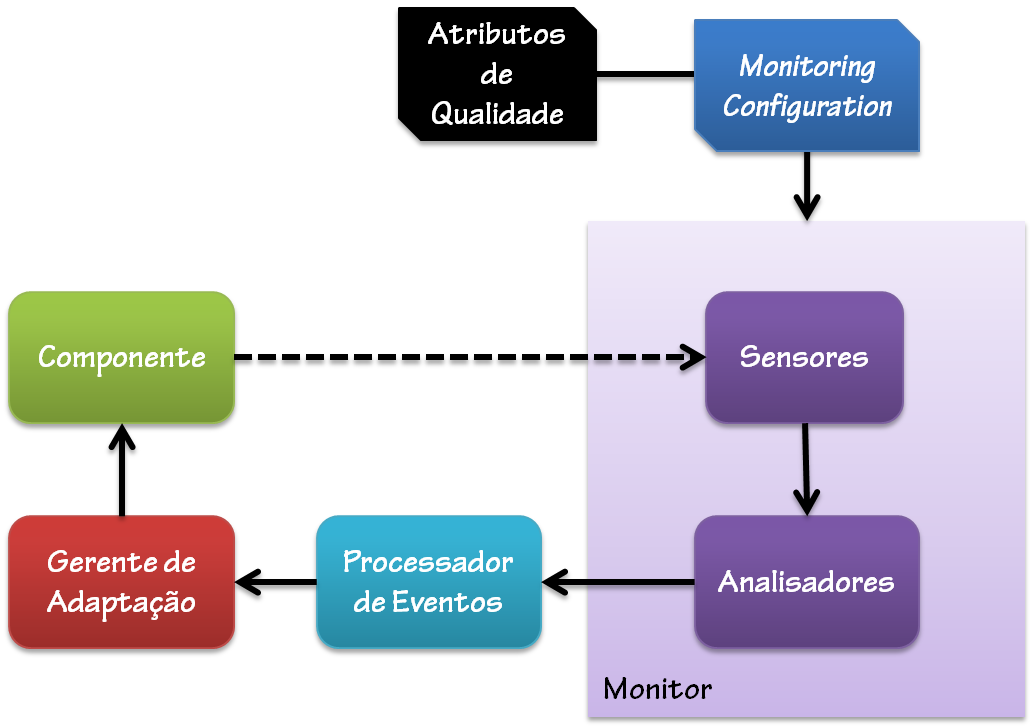
\includegraphics[width=11cm]{chapters/chapter3/monitor.png}
\caption{Sistema de Monitoração}
\label{fig:monitor}
\end{figure}

Porém, para prover adaptação dinâmica, o \textit{container} deve ser capaz de modificar-se sem provocar a interrupção do serviço. Para isso, a plataforma especifica a inclusão de uma camada de serviços de utilidade sobre a camada de composição de serviços e uma camada de adaptação, conforme a Figura \ref{fig:dsoa_arch}.

\begin{figure}[htp]
\centering
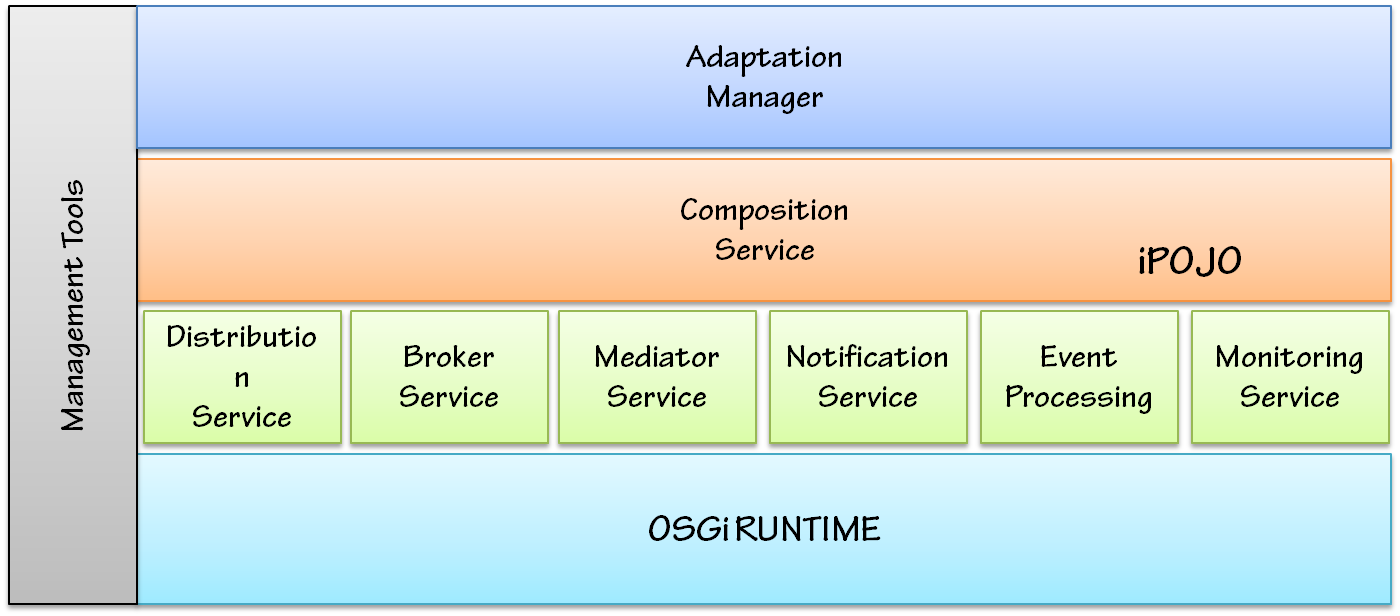
\includegraphics[width=13cm]{chapters/chapter3/dsoa-arch.png}
\caption[Arquitetura em Camdas DSOA]{Arquitetura em Camdas DSOA.}
\label{fig:dsoa_arch}
\end{figure}

\subsection{Componentes}
Nesta Seção, daremos uma uma visão geral de cada componente presente na arquitetura, identificando sua funcionalidade e suas características principais.

\subsubsection{\textit{Distribution Service}}
O serviço de distribuição é resposável por permitir que serviços disponibilizados no registro do \textit{runtime} OSGi local, sejam distribuídos como serviços remotos a outros \textit{runtimes}.

Esse serviços é provido através da utilização do DOSGi~\cite{dosgi}, que implementa um conjunto de serviços que provêem distribuição de serviços OSGi. 

Seu funcionamento baseia-se na ideia de um registro centralizado de serviços remotos, descritos como \textit{endpoints}, onde esses serviços são disponibilizados localmente através de ~\textit{proxies} que permitem o acesso ao ~\textit{endpoint}.

\subsubsection{\textit{Broker Service}}
%TODO

\subsubsection{\textit{Mediator Service}}
%TODO

\subsubsection{\textit{Notification Service}}
%TODO

\subsubsection{\textit{Event Processing Service}}
\label{subsec:cep}
%TODO

\subsubsection{\textit{Monitoring Service}}
\label{subsec:monit_serv}
%TODO

\subsubsection{\textit{Composition Service}}
%TODO

\subsubsection{\textit{Adaptation Manager}}
%TODO

\subsubsection{\textit{Management Tool}}
%TODO

